\chapter{Conclusion and Future Work}
\section{Conclusion}
The goal of this project was to introduce new intermediary service providers and replace the ID-centric append-only log from Secure Scuttlebutt with a feed bundle protocol. This extension or modification allows a much easier onboarding experience, since after signing a contract with an ISP the client is indirectly connected to all the ISP's servers. With the new introduce-detruce architecture, clients can connect and diconnect in a simple manner to new servers. Within this process new feed pairs are created, which bundle all the information for this specific connection. To ease the load on the wire and the process of replicationg every feed trough the ISP directly to the server, requests get multiplexed into a single feed pair between ISP and Server.
Since this system is developed newly completely out of the blue there are many ways to improve it, one of which is to use the feeds properties more to define the state of doneness inside the single log entries. There are still many ways to improve and expanded the system with important key features to generate a relieable client-ISP-server network. Some of them are discussed within the next section.
\section{Future Work}
Apart from improving the general system, we only ever looked at a single ISP with a single node to connect to with arbitrary many clients and servers connected. But in the real world this is not the case. There are many ISPs on the market and they have connectivity stations all around their country. So internet service providers (ISPs) and internet connectivity providers (ICPs) can be taken appart. Also contracts between ISPs could be possible. In the process of creating the simplified version of the feed bundle protocol, always a look at the big picture was takens and decisions were made with respect or kept in mind to this great picture.

\section{Combination of Log Entries}
Seen in the concept and the implementation, only a single new log entry is multiplexed into the ISP-server feed pair, resulting in a replication after each request. A diffrent approach can be made. We combine log entries in the multiplexing system. Meaning, instead of only one, a defined number of new log entries will be multiplexed to the server. This gives room for more efficient replication, since the whole feed gets replicated to the peer every time. Deriving from this the multiplexing feed pair can be splited up into arbitrary many sub feed pairs, linked to the priority of the request. 
\section{ISPs and ICPs}
As said, the ISP was always a single node, with contracts to clients and servers. But we could look at the ISP as a company with a net of ICPs where the physiscal connection to the servers and clients takes place. In simple terms, the client and server were indirectly ’connected’ over the ISP. The initial concept of the thesis was a peer-to-peer Internet Connectivity Provider (ICP) network where the ISP-Company distributes the feeds internally between the ICPs. In real life there is a contract to the ISP, e.g. Swisscom, and this very ISP has connectivity provider stations or nodes within the ISP newtork of ICPs. This means that a client has a connection with icp342 of Swisscom and the server has a contract with icp903. But both have a contract with Swisscom, who provides internal routing to pass information from icp342 to icp903.
\begin{figure}
    \centering
    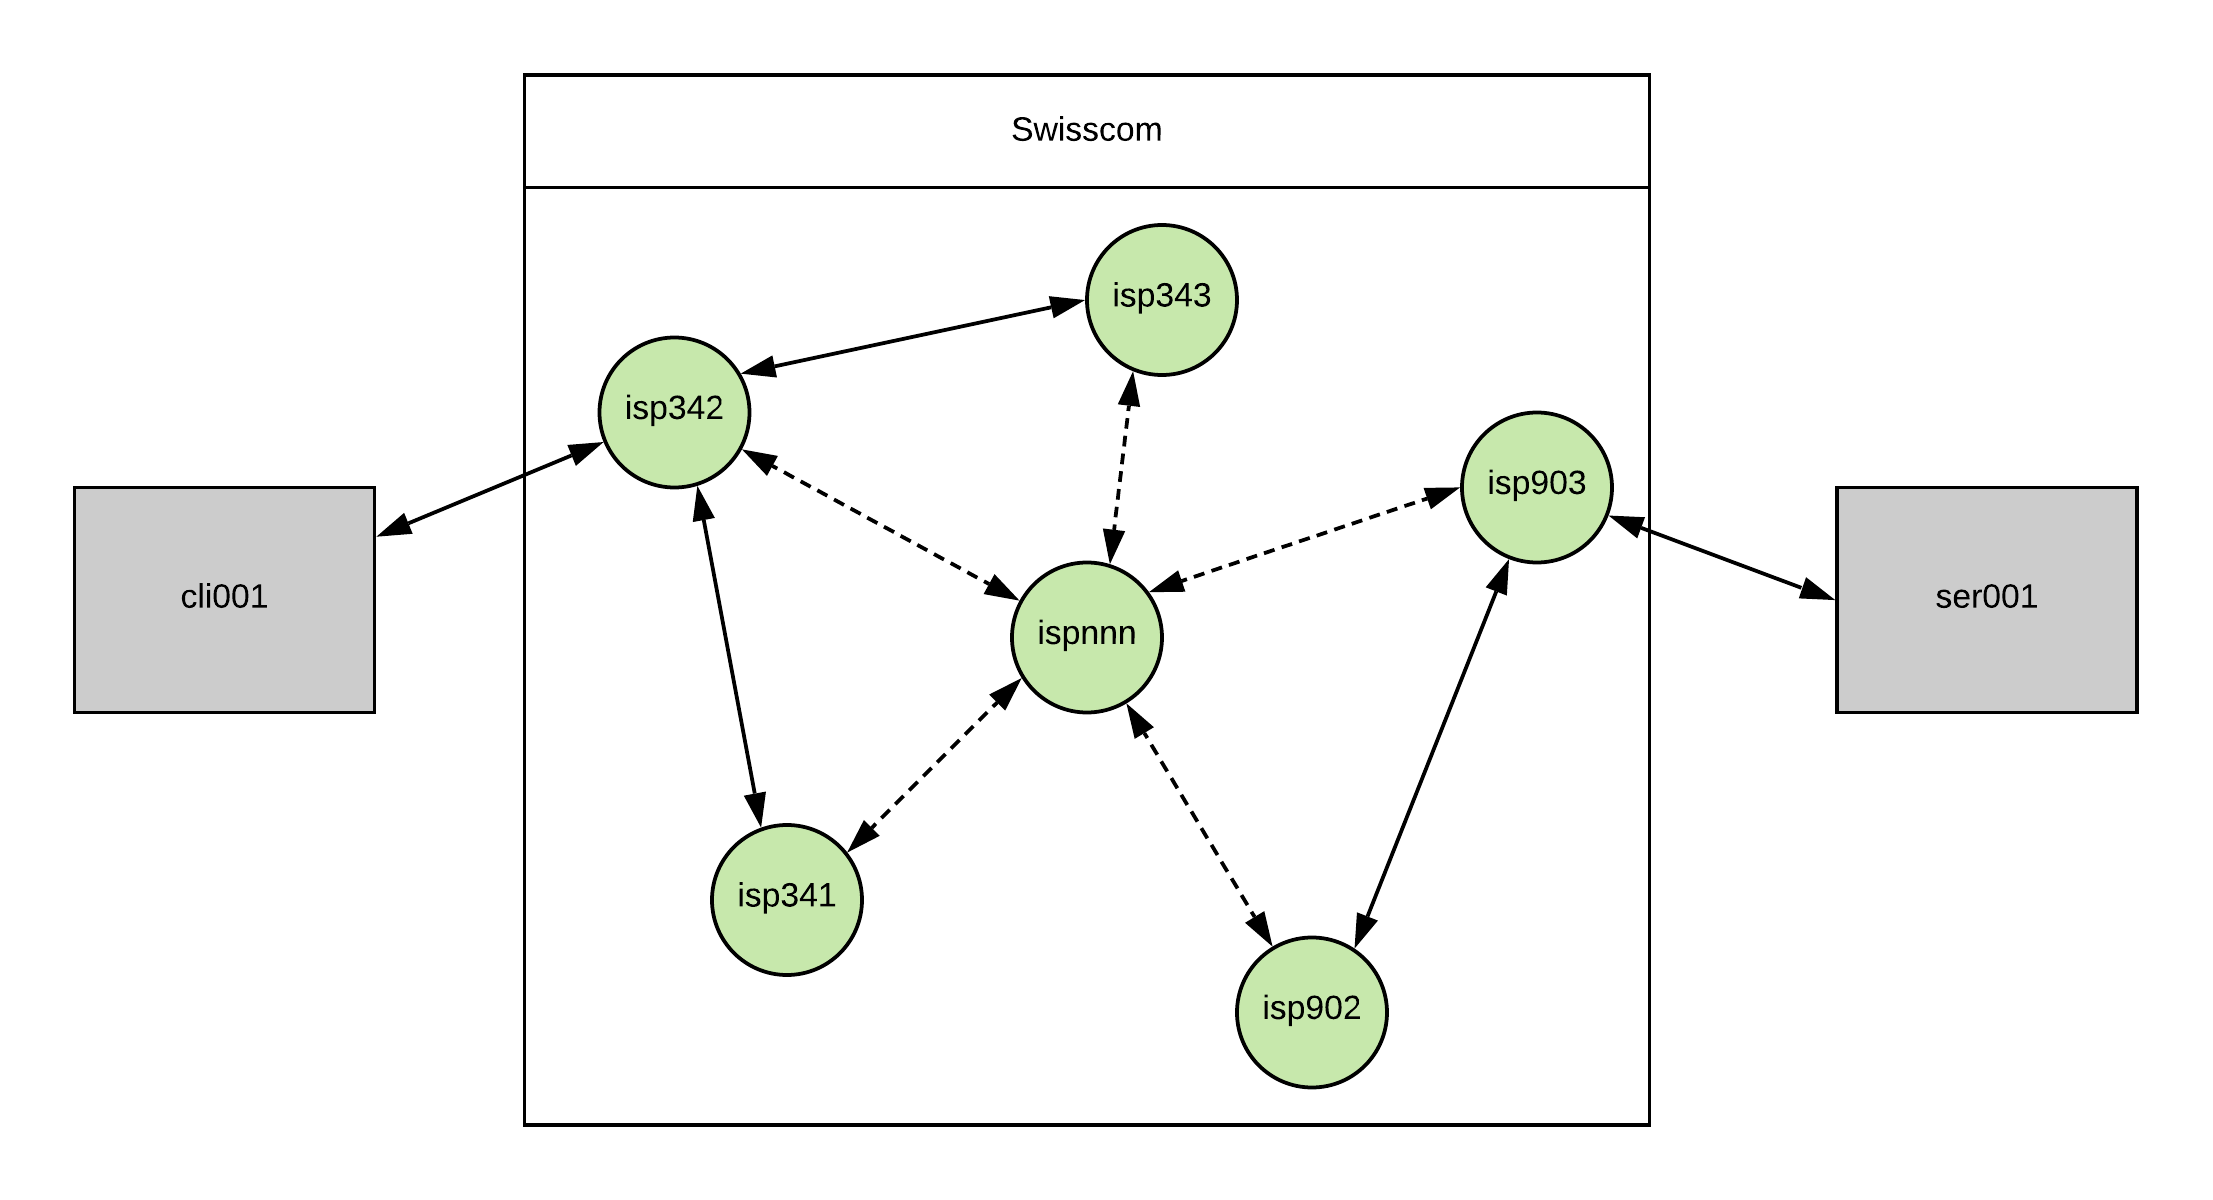
\includegraphics[width=0.9\textwidth]{p2p_contracts}
    \caption{A simplified contract network.}
    \label{fig:contract_network}
\end{figure}
Given this a new challenges emerge. How will the feeds be replicated? Either with the same approach as now where every ICP node stores a replication of each feed pair which it routes to the next node or only the multiplexed log entries will be appended to the ICP-ICP feed pair. Also it should be possible for a client to change the connectivity provider. If we say when traveling from Basel to Zurich also the ICP changes since they refer to antennas in the cities. There need to be new algorithms which handle these exact usecases.
\section{Contracts between ISPs}
Yet again, we can take this distribution to a next level where ISPs have contracts with ISPs. This leads to a way to bypass that every ISP needs to have a contract to every server. This has a very special impact on the system since then new contracts are generated, where the business aspect is not defined. The problem there is easier to explain by an example. If we say Google has a contract with Swisscom and Sunrise wants to have a contract to Google. There will be some money involved. Let's say Google pays Swisscom a hundred swiss francs for every introduced client. So Google has now the opportunity to make a contract with Sunrise, but they do not like each other very much and had difficulties earlier. So Google offers Sunrise fifty swiss francs per connected client. So Sunrise probably will not sign, since they have a good relationship with Swisscom. So now Swisscom offers Sunrise 75 swiss francs for every client they provide to Google. Now you see the dilemma. In the first scenario Google would make more profit, where as the second scenario is better for Swisscom and Sunrise. These dynamics are not simple, hence very interesting and have to be clarified. 
